\item A round cone \(A\) of mass \(m = 3.2 \, \text{kg}\) and half-angle \(\alpha = 10^\circ\) rolls uniformly and without slipping along a round conical surface \(B\) so that its apex \(O\) remains stationary (Fig. 1.36). The centre of gravity of the cone \(A\) is at the same level as the point \(O\) and at a distance \(l = 17 \, \text{cm}\) from it. The cone's axis moves with angular velocity \(\omega\). Find:
    \begin{center}
        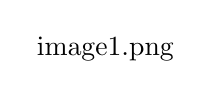
\begin{tikzpicture}
            \node at (0, 0) {{image1.png}};
        \end{tikzpicture}
    \end{center}
    \begin{enumerate}
        \item[(a)] the static friction force acting on the cone \(A\), if \(\omega = 1.0 \, \text{rad/s}\);
        \item[(b)] at what values of \(\omega\) the cone \(A\) will roll without sliding, if the coefficient of friction between the surfaces is equal to \(k = 0.25\).
    \end{enumerate}

\begin{solution}
    \begin{center}
        \begin{tikzpicture}
            \pic at (0, 0) {frame=3cm};
        \end{tikzpicture}
    \end{center}
    
    \begin{align*}
        \intertext{(a) Let us draw free body diagram and write Newton’s second law in terms of projection along vertical and horizontal directions, respectively,}
        N\cos{\alpha} - mg + fr\sin{\alpha} &= 0 \tag{1}\\
        fr\cos{\alpha} - N\sin{\alpha} &= m\omega^2l \tag{2}\\
        \intertext{From Eqs. (1) and (2)}
        fr\cos{\alpha}-\dfrac{\sin{\alpha}}{\cos{\alpha}}(-fr\sin{\alpha} + mg) &= m\omega^2l\\
        \intertext{So,}
        fr &= mg\left(\sin{\alpha} + \dfrac{\omega^2l}{g}\cos{\alpha}\right) \tag{3} \\
        &= 6 \text{ N (on substituting values)}
        \intertext{(b) For rolling, without sliding,}
        fr &\leq kN \\
        \intertext{but,}
        N &= mg\cos{\alpha} - m\omega^2l\sin{\alpha}\\
        mg\left(\sin{\alpha} + \dfrac{\omega^2l}{g}\cos{\alpha}\right) &\leq k\left(mg\cos{\alpha}-m\omega^2l\sin{\alpha}\right) \tag{using Eq. 3}\\
        \intertext{Rearranging, we get}
        m\omega^2l(\cos{\alpha} + k\sin{\alpha}) &\leq (k mg\cos{\alpha} - mg\sin{\alpha})\\
        \intertext{Thus,}
        \omega &\leq \sqrt{\dfrac{g(k-\tan{\alpha})}{(1+k\tan{\alpha})}l} = 2 \text{ rad/s}
    \end{align*}
\end{solution}
